\section{2d exploration strategies}
\tp{Ovdje bi bilo dobro staviti uvodnih par recenica koje ce se opisati u par recenica 2D exploration tj. da imamo vise robota koji imaju (nesavrsene) senzore, explored i unexplored space, donosimo odluku tocno gdje cemo ici u smjeru unexplored prostora. Reci da robot treba znati sto tocnije svoju poziciju sto tocnije. Mozes se i samo referencirati na postojecu Fig. 1 ili dodati novu. Mozes i navesti u kojem formatu zelimo dobiti mapu i koji se senzori najcesce koriste.
}
\tp{Također bi trebalo slikovito prikazati strukturu rjesenja (nesto kao Fig 3., ali malo opcenitije). Ovo mozes za prezentaciju, ne trebas sad.}

Exploration algorithms can be grouped into centralized and decentralized. In \st{the}  centralized approaches, each robot receives tasks from a single central \emph{leader}, which runs the overall planning algorithm, and afterwards the robot sends its info back to the leader. {\color{red}A} centralized assignment may be less practical due to communication limits (\cite{Dias2000}), robustness issues (\cite{Dias2006}), or {\color{red}the} time required for algorithm execution and scalability (\cite{Julia2012}). An advantage of centralized approaches is that optimal plans can be found (\cite{Yan2011}). For instance, Sharma et al. \cite{SharmaHonc2016} used a centralized exploration \st{approach} {\color{red}strategy} based on routing priority. The algorithm keeps track of the frontiers, assigning them to robots whenever they fall into {\color{green}a trap situation}.

\tp{Sto je trap situation, mozda bolje koristiti neki drugi izraz}

In contrast to centralized approaches, in a decentralized approach, the robots are completely ({\color{red} or at least partially}) independent throughout the exploration process. Each robot has its own local knowledge of the world and can decide its future actions by taking into account its current context and tasks, its own capacities and the capacities of the other robots. \st{through a negotiation process} (\cite{Yan2013}) {\color{red} Robot send and received information to/from other robots in its communication range}. Moreover, it typically has better reliability, flexibility, adaptability and robustness (\cite{Zlot2002}). 
 
There are several representative approaches from \st{the} both centralized and decentralized 2D exploration strategies described in the following text. 

\subsection{Nearest Frontier Approach} 
An unexplored area is usually represented using an occupancy grid map introduced by \cite{Moravec}. While a robot moves, an occupancy likelihood for each cell of the grid is updated with the information \st{of} {\color{red} gathered by} sensors. Depending on this occupancy likelihood, cells can be classified as free, occupied or unknown (Fig. \ref{fig:environment}). Using an occupancy grid, a robot can reach an unexplored zone navigating to the frontier cells that separate the free cells from the unknown cells known as \textit{frontiers} \cite{Yamauchi1997}. A general frontier exploration diagram is shown in Fig. \ref{fig:flow_diagram}.
\begin{figure}[t!]
	\centering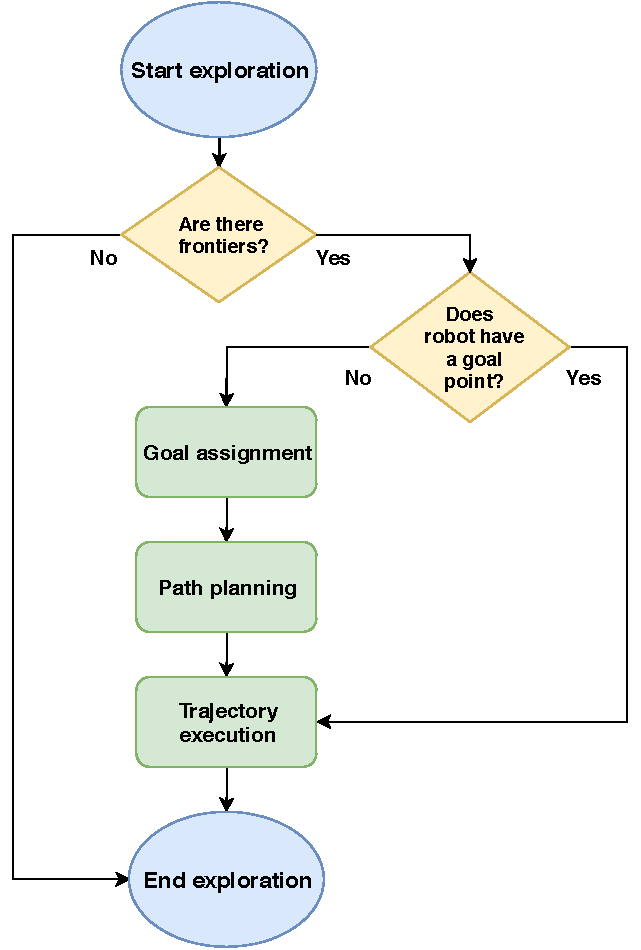
\includegraphics[width=0.85\columnwidth]{./pictures/flow_diagram.pdf}
	\caption{Flow diagram for the frontier exploration strategies. \In case a robot {\color{red}is idle} (does not have a goal point), a new goal is computed, assigned, a path to the assigned goal is obtained and a trajectory executed.}
	\label{fig:flow_diagram}
\end{figure}
Yamauchi's technique consists in selecting the shortest path to the nearest frontier. In this way, the target cell selected by this technique $t_{NF}$ is:
\begin{equation}
t_{NF} = \argmin_{a \in F} L(a), 
\label{equation:t-nf}
\end{equation}
where $L(a)$ represents the length of the shortest path to reach the cell $a$ ($a_{i}$, $a_{j}$) and $F$ the subset of the frontier cells \cite{Julia2012}. As it can be noticed, (\ref{equation:t-nf}) takes into account the cost of reaching a frontier cell and does not provide any coordination mechanism. In case a single robot system is extended to a multi-robot system, robots may select the same frontier if they are situated in nearby positions. For instance, \cite{Yamauchi1998} extended his nearest frontier approach to multiple robots using global maps built by each robot with the information provided by all robots. Since robots share the acquired information, exploration is cooperative, \st{but robot movements are uncoordinated} {\color{red}however, the selection of target points remains uncoordinated}. When the robots are in \st{close positions} {\color{red}the vicinity of each other} it is likely that they {\color{red}are going to} choose the same frontier {\color{red}point or region} to explore if no other coordination mechanisms are considered.

Frontier exploration strategies are also extended to a multi-robot system in \cite{Simmons2000} and \cite{Burgard2005}. Simmons \cite{Simmons2000} used a semi-distributed model where a centralized module integrates local data from a team of robots. The team used a probabilistic technique to build a global map in a coordinated fashion. \st{Due to the problem of absolute positioning techniques in indoor environments, robots must estimate their local pose in an environment, leading to odometry errors.} {\color{red}To account for odometry errors in determination of absolute robot position}, Simmons used probability calculations to estimate the local pose of each robot, and built a global map by joining each individual robots local map. 
While Simmons \cite{Simmons2000} implements coordination between robots by sharing of map information and reducing the utility of frontier points in the vicinity of an allotted point, Burgard \cite{Burgard2005} came up with an elegant bidding process. 

A dense frontier points detection method implemented by Orsulic (\cite{Orsulic2019}) is an extension to Google Cartographer (\cite{Hess2016}) that has achieved good results in terms of wall-time per frontier update, which greatly speeds up {\color{red}the} exploration process. Orsulic used nearest frontier approach in order to explore an area. 

Rekeleitis \cite{Rekeleitis2000} covered terrains with multiple robots where at least one robot was stationary and posed as an observer. In \cite{Fox2006} a decision theoretic approach to multi-robot exploration was presented where the main problem was to decide whether a robot should explore the terrain or \st{to} verify the hypothesis of other robots whose states are not mapped into a common reference frame. The nearest unexplored region technique is also used by Wullschleger \cite{Wullschleger99}, Santosh \cite{Santosh2008}, Murphy and Newman \cite{Murphy2008}, to name a few \st{more}.

\subsection{Cost-Utility Approach}
Generally, in a cost-utility approach a goal point maximizes the benefit {\color{red}(difference)} between utility and cost. The utility is {\color{red}calculated as the expected information gain from visiting the position of the goal point} \st{measured in terms of the expectation of the information incorporated to the occupancy map from the position of the goal point}. An example of cost-utility approach was presented by González-Baños and Latombe \cite{GonzlezBaos2002}. Frontier cells are designated as candidate destinations and the benefit $B_{CU}(a)$ to reach a candidate cell a is evaluated according to the following expression:
\begin{equation}
B_{CU}(a) = U(a) - \lambda_{CU}C(a),
\label{equation:cost-utility}
\end{equation}
where $U(a)$ is a utility function, $C(a)$ is a cost function and $\lambda_{CU}$ is a constant that adjusts the relative importance between both factors \cite{Julia2012}. Utility and cost functions are expressions normalized in the range $\left[0, 1\right]$ that are calculated as follows:
\begin{equation}
U(a) = \frac{U_{nex}(a, R_{s})}{\pi R_{s}^{2}},
\end{equation}
\begin{equation}
C(a) = \frac{L(a)}{max_{b \in F}L(b)},
\end{equation}
where the function $U_{nex}(a, R_{s})$ is \st{the result of counting} the number of unexplored cells in the range of the sensor from cell $d$ {\color{green}cell $a$?}, \st{being} $R_{s}$ {\color{red}being} the maximum range of the sensor expressed in cell units.
Then, the target cell $t_{CU}$ is chosen as the one that maximizes the utility-cost relation \cite{Julia2012}:
\begin{equation}
t_{CU} = \argmax_{a \in F} B_{CU}(a).
\end{equation}
Similar to the work proposed by Simmons, Burgard \cite{Burgard2000} introduced \st{some} coordination by means of reducing \st{a determined initial utility given to each frontier depending on the likelihood of being in the sensor range from other frontiers that have been assigned to other robots.} {\color{red} the utility of a frontier point depending on the likelihood that it is in the vicinity of a frontier point already-assigned to another robot.} The assignment of frontiers to robots is made {\color{red}in a greedy manner} (sequentially) using a cost-utility approach with the length of the minimum path {\color{red}{to a frontier point}} as cost. It is assumed that robots know each others relative positions. {\color{green}The algorithm determines optimal target points for each robot that increase the coverage by the maximum amount at that time period - Ovo je nejasno napisano, napisi tocno sto se odvija, npr. In each iteration of the assignment algorithm, the best robot-to point assignment is calculated using cost-utility. The chosen robot is not considered in the next iteration - ne znam tocno kako ide.}. Moreover, Burgard in \cite{Burgard2005} suggested that the assignment of frontiers to robots could be optimized using the Hungarian method \cite{Kuhn1955} instead of the sequential assignment.

Another example of cost-utility model is given in \cite{Umari2017}, where a frontier detection method is based on Rapidly Exploring Random Trees (RRTs). Umari defines revenue from a frontier point as a combination of an information gain and navigation cost. 
 
Bhattacharya et al. \cite{Bhattacharya2013}, \cite{BhattacharyaGhrist2013} focused on the use of cost functions related to information theory, casting the exploration problem as a minimization of map entropy. Authors combined this approach with a grid-based map decomposition with an entropy minimization which results in complete coverage of a known map and full exploration if the scenario is unknown. 

\subsection{Market-Based Approach}
\tp{Po meni su ovo sve cost-utility problemi, a onda se dalje dijele na 1)Greedy/simple 2)Market-based 3) Optimization based - jesam li u krivu?}

The general concept of the market-based approaches includes independence of robots in terms of planning, and the ability of robots to take team resources into account.
Relatively close to Burgard's approach in \cite{Burgard2000}, Zlot \cite{Zlot2002} uses a market architecture for the multi-robot mapping and exploration problem that aims to minimize an overall exploration time. In market-based coordinated approach each robot contains a list of goal points and \st{profits} {\color{red}benefits} associated with (\ref{equation:cost-utility}). Each robot selects the most profitable target as destination and when after reaching a current goal point, a robot initiates an auction. For each point in auction, each robot makes a bid with its current profit aiming to minimize own travel distance and maximize new area information.

It is shown in \cite{Dias2003} when different team sizes are included, a market method has an advantage over a centralized approach in terms of travelled distance. 

Michael et al. \cite{Michael2008} proposed a marked-based coordination protocol where robots are able to bid for task assignment with the assumption that every robot has knowledge of the maximum number of robots that any given task can accommodate. Each auction is performed among neighboring groups of robots and requires only local communication.

Sheng et al. \cite{Sheng2006} proposed an algorithm based on a distributed bidding model to coordinate the movement of multiple robots with limited communication range. The bidding algorithm takes into consideration distances between robots and a map synchronization mechanism reduces the exchanged data volume when robot subnetworks merge.

\subsection{Decentralized Coordinated Approach}

Pereira et al. \cite{Pereira2015} proposed a new exploration and mapping strategy, which relies on individual decision rules and communication of topological maps to achieve efficient and fast mapping. In this distributed strategy each robot broadcasts a graph representing the topological map, which can be transmitted to robots that are not within the communication range (through other robots in a system). 

Decentralized coordinated approach described in \cite{Colares2016} showed how exploration efficiency can be greatly improved. Authors presented a decentralized approach for multi-robot exploration that leverages the classical frontier based methods. The strategy took into consideration a utility function (the information gain) and the distance costs of frontiers. In that manner, robots are able to coordinate themselves and avoid the exploration of redundant areas by exchanging information and merging maps.
\tp{Koja je razlika u odnosu na Burgarda npr}

Lopez-Perez et al. \cite{LopezPerez2018} proposed a new method to explore unknown areas by using a scene partitioning scheme and assigning weights to the frontiers between explored and unknown areas. Authors presented a distributed algorithm, which reduces the number of communications between robots as well as the time needed to explore unknown regions and the distance traveled by each robot. Algorithm implemented by Benkrid and Achour \cite{Benkrid2017} also assigns weights to frontier cells, but, on the other hand, depends on the energy of the battery of each robot.

Another interesting approach is proposed by Faigl et al. \cite{Faigl2015} where a goal assignment is solved as task-allocation problem, where goal locations are repeatedly determined during the exploration. 

In the described approaches, the main focus is improving the next action in order to explore an unknown area as fast as possible. Authors aimed to reduce a distance traveled by the robots as well as information shared between robots. This work motivated us to implement a decentralized strategy for autonomous multi-robot frontier exploration and mapping of an unknown area. 

Overview of our system is given in Fig. \ref{fig:exploration-strategy}. The system consists of a centralized part (Simultaneous Localization and Mapping (SLAM), frontier detection and frontier points filter), which runs on a dedicated computer and a decentralized part (Exploration strategy and navigation), which runs on each robot. 

In our approach a robot team simultaneously explores the environment, discovers frontier points and shares information in order to become dispersed throughout the environment. During the exploration, information exchanged between the robots is limited to data containing robot positions and current robot target points. The main goal of the approach is to allocate the robots to target frontier points in a way which minimizes the overall exploration time. Moreover, a robot team at the same time creates a common map of the environment. 

Our approach is a hybrid one - the robots can independently decide towards which target point to navigate using an optimization procedure, while having common knowledge of all target frontier points and sharing information on their position and current goals. We use slightly different objective functions for frontier points assignment called \textit{weight function}, which are a combination of frontier point cost, utility of reaching the target point and \textit{frontier occupancy function}. We also cluster frontier points to get a problem of manageable size and thus enable application of known optimization algorithms. 
Our approach is hybrid in a manner that target point assignment process and navigation are fully decentralized and event-based, that is, each robot team member makes an individual decision on the next target point each time it reaches the previous one. On the other side, SLAM extended with frontier detection and filter module are a centralized part of the exploration and mapping process.
\tp{Slobodno stavi ovdje i neke rezultate tj. grafove}

\begin{figure}[t!]
	\centering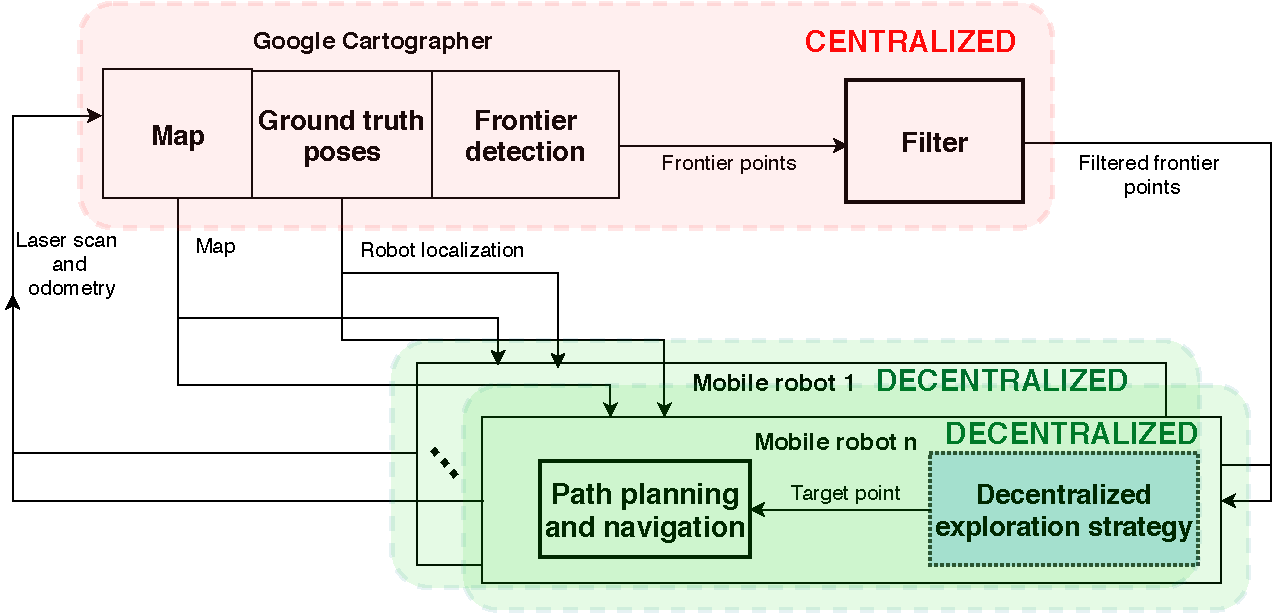
\includegraphics[width=1.0\columnwidth]{./pictures/diagram_exploration.pdf}
	\caption{Overall schematic diagram of the decentralized exploration and mapping process for $n$ robots in the simulator. Google Cartographer SLAM and filter module (highlighted in red) generate filtered frontier points that are (currently) the centralized part of exploration and mapping process. The exploration strategy, path planning and navigation module (highlighted green) are decentralized parts that generate $n$ outputs and create a common map.}
	\label{fig:exploration-strategy}
\end{figure}


\begin{algorithm}[b!]
	\While{Unexplored}{
		\If{Request}{
			Send position and current target point to the other mobile robots\;
		}
		\If{Robot has reached the previous target point}{
			Request positions and current target points from other mobile robots\;
			Calculate weight function\;
			Hungarian algorithm\;
			\textbf{return} Robot is assigned to frontier point\;
		}
	}
	\label{algorithm1}
	\caption{Decentralized strategy for multi-robot exploration.}
\end{algorithm}


Our decentralized strategy executes during the robot motion and there are steps for each robot to be executed (\textbf{Algorithm 1}). All frontier points are visible to all robots.
When a robot is assigned to a frontier point according to line 8 in \textbf{Algorithm 1}, the robot starts to follow the planned path and navigates to the target frontier point. At the moment when the robot reaches the target point (mission is over), a request is sent to other robots to get their positions and current target points. Calculated weight function are an input to Hungarian algorithm. 
The Hungarian algorithm is described in \cite{Kuhn1955} and tested in \cite{Kulich2015}. Initially, the Hungarian algorithm assumes that the number of frontier points is the same as the number of robots. Due to the fact that there are usually fewer robots than frontier points, virtual robots are added and then skipped during the process of assignment and exploration. 

The described process executes until the whole environment is explored and a complete  map of the environment is generated.

This approach is not only restricted to Google Cartographer SLAM and dense frontier detection, but may also be applied to different multi-robot systems. This strategy has resulted in improved behaviour in terms of exploration time compared to a state-of-the-art strategy in terms of exploration time. 


